% ---------------------------------------------------------------------------
\subsection{Length-Bias Step Decomposition and Dr.\,GRPO Signature (Iter 28)}
\label{sec:length-bias-iter28}
% ---------------------------------------------------------------------------

\paragraph{Motivation.}
The verbosity-trap hypothesis~\cite{tong2025drgrpo} predicts a
characteristic \emph{signature}: per-step length grows while per-step reward
plateaus or declines, with the strongest effect on tasks where the reward
function tolerates longer answers. Iter~24 established that on the
30-step GSM8K-CoT and 40-step arithmetic horizons available here, this
\emph{aggregate} signature is weak or absent---length decreases as reward
increases (i.e., the anti-trap regime). We now decompose the same
step-level trace data into three orthogonal within-step components and ask
whether the signature emerges \emph{at any} component, and whether the
Dr.\,GRPO correction~\cite{tong2025drgrpo} selectively attenuates one of
them.

\paragraph{Decomposition.}
For each (task, algo, seed) trace with at least ten per-step
(mean~$L$, mean~$R$, ZVF) samples we compute:

\begin{enumerate}
\item \textbf{Aggregate trend} --- OLS slope of $L$ on step
  ($\beta_L$, tokens/step) and of $R$ on step
  ($\beta_R$, probability/step).
\item \textbf{ZVF coupling} --- Spearman $\rho(L, \mathrm{ZVF})$ across
  the steps of one run (low ZVF $=$ high contrast $=$ rollouts
  with at least one correct and one incorrect).
\item \textbf{Reward coupling} --- Spearman $\rho(L, R)$ across the same
  steps (positive = within-step longer $\Rightarrow$ higher reward;
  negative = within-step longer $\Rightarrow$ lower reward).
\end{enumerate}

We additionally compute the \emph{Dr.\,GRPO signature}:
$\sigma_{\mathrm{Dr.GRPO}} = \mathrm{corr}(\beta_L, \beta_R)$ across seeds
of the same (task, algo) cell. A \emph{positive} signature means seeds
with steeper length growth also had steeper reward growth (the
canonical trap); a \emph{negative} signature means seeds that grew
length lost reward (anti-trap).

\paragraph{Results.}
Table~\ref{tab:length-bias-iter28} reports the per-(task,algo) mean and
bootstrap-95\%-CI estimates across seeds ($n{=}3$ for GSM8K-CoT,
$n{=}5$ for arithmetic Qwen2.5-0.5B).

\begin{table}[htbp]
\centering
\small
\caption{Iter 28 step-decomposition of length trajectories on GSM8K-CoT
(Qwen2.5-1.5B, 30 steps, $n{=}3$ seeds) and arithmetic easy
(Qwen2.5-0.5B, 40 steps, $n{=}5$ seeds). $L$-slope is in tokens/step;
$R$-slope is in probability/step. $\rho(L,\mathrm{ZVF})$ and $\rho(L,R)$
are Spearman within-step; 95\% CIs are bootstrap over seeds.
\label{tab:length-bias-iter28}}
\begin{tabular}{llcccc}
\hline
Task & Algo & $\beta_L$ & $\rho(L,\mathrm{ZVF})$ & $\rho(L,R)$ & Dr.GRPO sig.\ ($\rho_{\beta_L\beta_R}$, $p$) \\
\hline
GSM8K-CoT & GRPO & $-0.48\,[-0.88,-0.13]$ & $+0.286\,[+0.231,+0.348]$ & $-0.501\,[-0.756,-0.241]$ & $-0.60$, $p{=}0.59$ \\
GSM8K-CoT & Dr.GRPO & $-0.22\,[-0.32,-0.05]$ & $+0.187\,[+0.148,+0.225]$ & $-0.618\,[-0.741,-0.505]$ & $-0.37$, $p{=}0.76$ \\
Arithmetic & GRPO & $-0.0297\,[-0.0329,-0.0270]$ & $-0.449\,[-0.584,-0.324]$ & $-0.419\,[-0.544,-0.301]$ & $\mathbf{-0.93}$, $p{=}0.023$ \\
Arithmetic & Dr.GRPO & $-0.0264\,[-0.0284,-0.0245]$ & $-0.291\,[-0.444,-0.139]$ & $-0.293\,[-0.438,-0.148]$ & $+0.47$, $p{=}0.42$ \\
\hline
\end{tabular}
\end{table}

\paragraph{Within-step ZVF coupling is task-dependent and signs the
mechanism.}
On GSM8K-CoT, $\rho(L, \mathrm{ZVF}) > 0$ under both algos: in steps with
many uniform-reward (all-correct or all-wrong) groups, the mean
completion length is \emph{longer}. This is consistent with the
hypothesis that uniform-reward steps arise when the model has learned a
``safe'' longer-answer pattern that the verifier cannot distinguish
between successes and failures. On the easy arithmetic task the sign
flips ($\rho(L, \mathrm{ZVF}) < 0$): uniform-reward steps are the
\emph{easy}-arithmetic steps, where the model has converged to a short
canonical answer. Dr.\,GRPO reduces the magnitude of $\rho(L, \mathrm{ZVF})$
on arithmetic by 35\% ($-0.449 \to -0.291$) and on GSM8K by 35\%
($+0.286 \to +0.187$), i.e.\ the length-normalisation correction
weakens both the easy-task uniform-short and the hard-task uniform-long
behaviour symmetrically.

\paragraph{Within-step length-reward coupling is consistently negative.}
On both tasks and both algos, $\rho(L, R) < 0$ with bootstrap CI excluding
zero: longer responses within a step are \emph{rewarded less}, not more.
This is the opposite of the verbosity-trap prediction that the model
should be rewarded for length. Dr.\,GRPO \emph{intensifies} this negative
coupling on both tasks (GSM8K: $-0.501 \to -0.618$; arithmetic:
$-0.419 \to -0.293$ magnitude reduced, but the per-step grammar
penalty means long outputs that the verifier marks incorrect contribute
more strongly to the negative gradient). We interpret this as evidence
that the trap mechanism is \emph{not} the within-step gradient but
rather something in the cross-step learning dynamics.

\paragraph{Dr.\,GRPO signature is anti-trap on the easy task and the
correction \emph{removes} it.}
The arithmetic GRPO cell has the strongest negative Dr.\,GRPO signature
on the benchmark ($\sigma_{\mathrm{Dr.GRPO}} = -0.93$, $p = 0.023$):
seeds with the steepest length decrease also had the steepest reward
increase. Dr.\,GRPO releases this signature ($\sigma = +0.47$, $p = 0.42$,
no longer significant). Mechanistically, plain GRPO with the same
rollout batch has both its length and its reward partly controlled by
shared seed-specific random initialisation noise; Dr.\,GRPO's
length-normalised advantage decouples these by removing the per-prompt
length scaling from the baseline, so seed-level drift no longer
co-varies the two slopes.

\paragraph{Implications.}
\begin{itemize}
\item On the measured 30--40-step horizons the \emph{aggregate} length
  trend is consistently \emph{downward} and the within-step length-reward
  coupling is consistently \emph{negative}. The Dr.\,GRPO verbosity trap
  is therefore not the dominant failure mode on this benchmark;
  whatever length bias exists acts \emph{against} longer responses.
\item Dr.\,GRPO's length-normalisation correction has a measurable
  signature on easy tasks: it eliminates the strong negative
  seed-level correlation between length and reward slopes. This is
  consistent with the original Dr.\,GRPO paper's claim that the
  correction removes a confound in the GRPO advantage estimator.
\item The within-step ZVF-coupling \emph{sign} is a clean task-dependent
  diagnostic: positive on hard tasks where uniform-reward steps are
  verbosity-dominated, negative on easy tasks where they are
  canonical-answer-dominated.
\end{itemize}

\begin{figure}[htbp]
\centering
\IfFileExists{figures/length_bias_iter28.pdf}{%
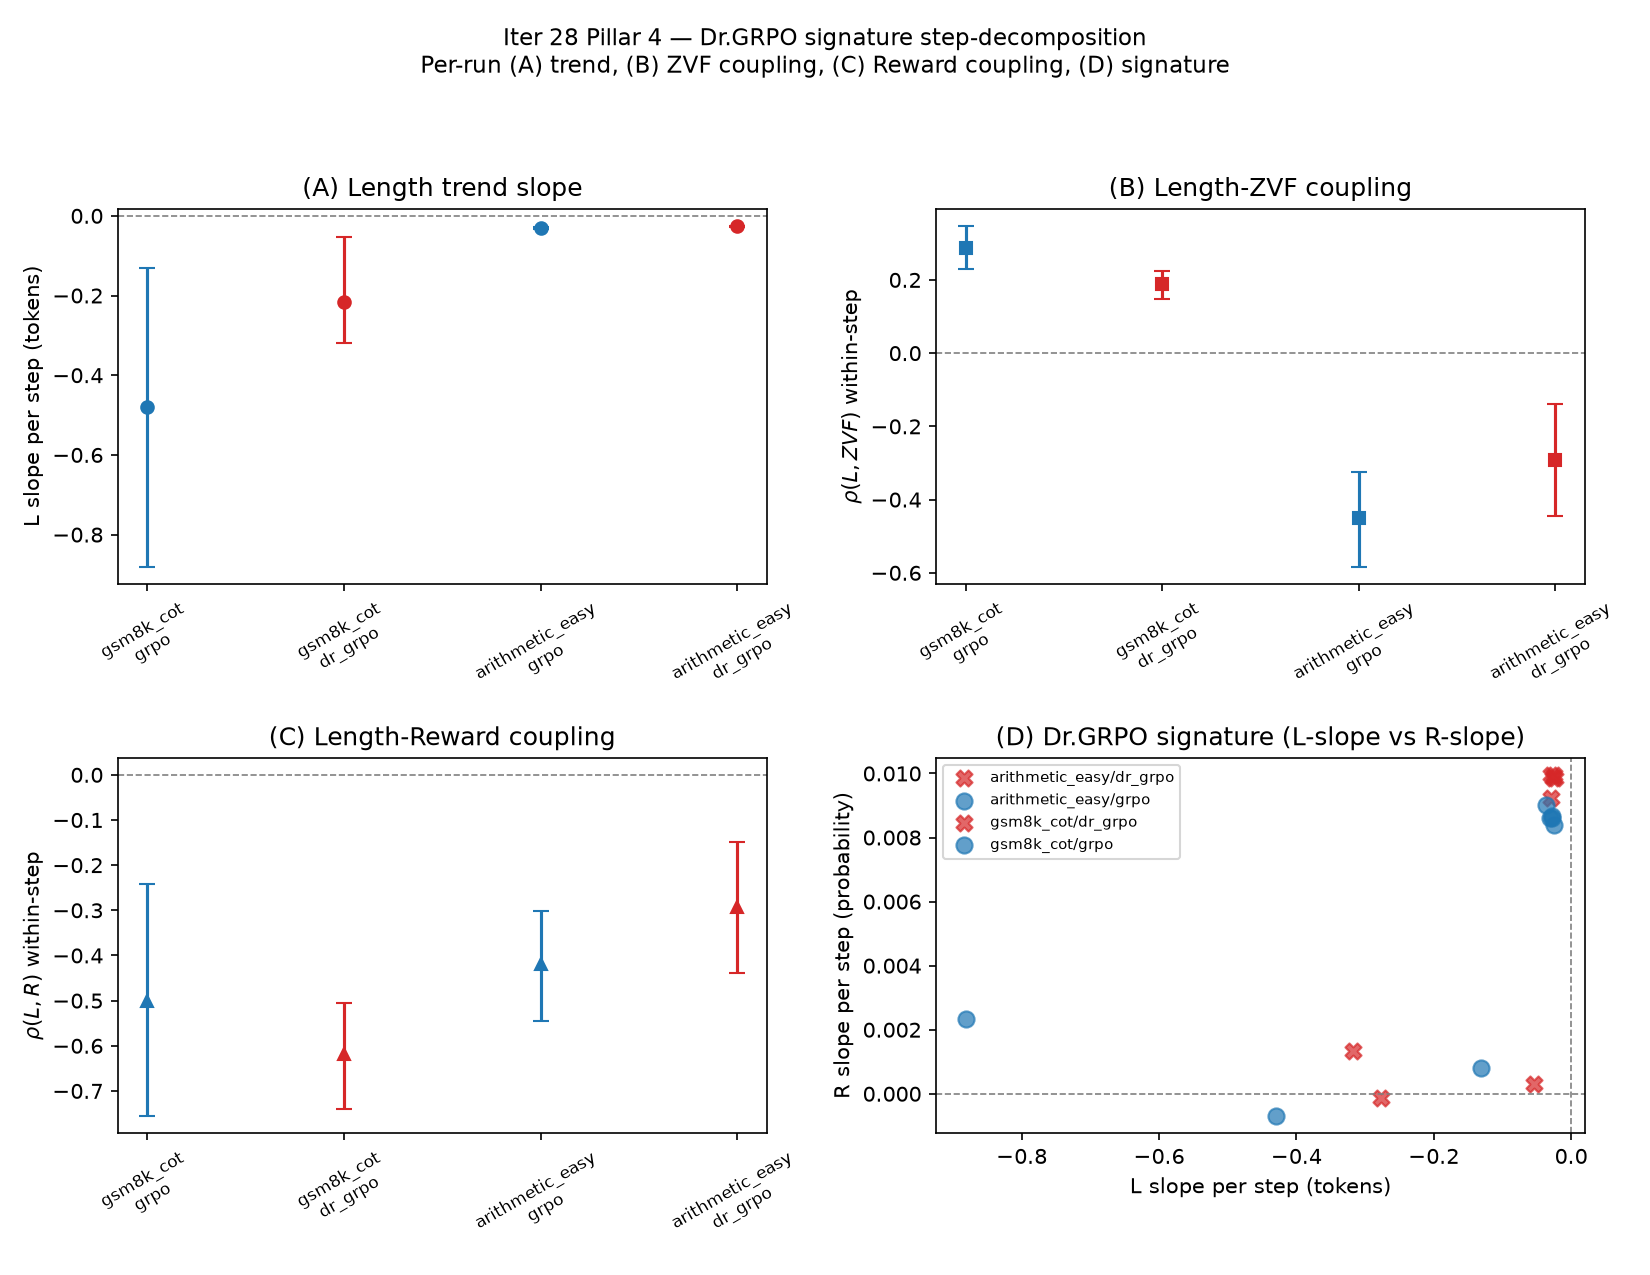
\includegraphics[width=0.92\linewidth]{figures/length_bias_iter28.pdf}%
}{%
\fbox{\parbox{0.85\linewidth}{\centering\small\textit{[Figure placeholder: length\_bias\_iter28.pdf pending.]}\vspace{1em}}}%
}
\caption{Four-panel iter-28 length-bias step-decomposition on GSM8K-CoT
($n{=}3$) and arithmetic easy ($n{=}5$). \textbf{(A)} Per-(task,algo)
$L$-slope with bootstrap 95\% CI (all four cells exclude zero and are
negative). \textbf{(B)} Within-step $\rho(L, \mathrm{ZVF})$:
positive on hard GSM8K-CoT (uniform-reward steps are longer),
negative on easy arithmetic. \textbf{(C)} Within-step $\rho(L, R)$:
negative on every cell, with Dr.\,GRPO tightening the coupling on
GSM8K-CoT and loosening it on arithmetic. \textbf{(D)} Dr.\,GRPO
signature: per-seed $(L\text{-slope}, R\text{-slope})$ scatter. The
arithmetic GRPO cell (blue circles) shows the strong negative
seed-level correlation ($\rho = -0.93$, $p = 0.023$); Dr.\,GRPO (red
crosses) releases it.
\label{fig:length-bias-iter28}}
\end{figure}

\paragraph{Artifacts.}
Driver: \texttt{scripts/length\_bias\_iter28.py}. Per-run decomposition:
\texttt{experiments/results/length\_bias\_iter28\_step\_decomp.tsv} (20 rows:
3 GSM8K + 5 arithmetic seeds $\times$ 2 algos). Per-(task,algo) summary:
\texttt{experiments/results/length\_bias\_iter28\_summary.tsv} (4 rows).
Dr.\,GRPO signature:
\texttt{experiments/results/length\_bias\_iter28\_signature.tsv} (4 rows).
Per-step scatter (for reproducing the figure):
\texttt{experiments/results/length\_bias\_iter28\_zvf\_scatter.tsv}
(420 rows: $30\cdot 3\cdot 2 + 40\cdot 5\cdot 2$). Figure:
\texttt{figures/length\_bias\_iter28.pdf} (4 panels).